\documentclass[11pt,a4paper]{article}
\usepackage[a4paper,margin=2.4cm]{geometry}
\usepackage[T1]{fontenc}
\usepackage[utf8]{inputenc}
\usepackage{amsmath,amssymb,amsthm}
\usepackage{booktabs,array,enumitem}
\usepackage{tikz}
\usetikzlibrary{arrows.meta,calc,positioning}
\usepackage{pgfplots}
\pgfplotsset{compat=1.17}
\usepackage[most]{tcolorbox}
\usepackage[colorlinks=true,linkcolor=blue!50!black,urlcolor=blue!50!black]{hyperref}

\newcommand{\R}{\mathbb{R}}
\newcommand{\N}{\mathcal{N}}
\newcommand{\dq}{\dot q}
\DeclareMathOperator{\SO}{SO}
\DeclareMathOperator{\rank}{rank}

% ---------- theorem-like environments (shared counter, boxed) ----------
\theoremstyle{definition}
\newtheorem{theorem}{Theorem}[section]
\newtheorem{definition}[theorem]{Definition}
\newtheorem{lemma}[theorem]{Lemma}
\newtheorem{proposition}[theorem]{Proposition}
\newtheorem{corollary}[theorem]{Corollary}
\newtheorem{example}[theorem]{Example}
\newtheorem{algorithm}[theorem]{Algorithm}

\tcbset{thmbox/.style={breakable,enhanced jigsaw,colback=white,colframe=black!65,
  boxrule=0.6pt,arc=1.5pt,left=5pt,right=5pt,top=3pt,bottom=3pt,before skip=9pt,after skip=9pt}}
\tcolorboxenvironment{theorem}{thmbox}
\tcolorboxenvironment{definition}{thmbox}
\tcolorboxenvironment{lemma}{thmbox}
\tcolorboxenvironment{proposition}{thmbox}
\tcolorboxenvironment{corollary}{thmbox}
\tcolorboxenvironment{example}{thmbox}
\tcolorboxenvironment{algorithm}{thmbox}

% ---------- blue Intuition box ----------
\newtcolorbox{intuition}[1][Intuition]{breakable,enhanced jigsaw,
  colback=blue!5,colframe=blue!60!black,coltitle=white,fonttitle=\bfseries,
  title={#1},boxrule=0.6pt,arc=2pt,left=6pt,right=6pt,top=3pt,bottom=3pt,
  before skip=9pt,after skip=11pt}

\title{\textbf{Autonomous and Mobile Robotics}\\[2pt]
\large Kinematic Models of Wheeled Mobile Robots\\[2pt]
\normalsize Lecture notes -- part 3 (from the handwritten notes \texttt{AMR03.pdf})}
\author{}
\date{}

\begin{document}
\maketitle
\tableofcontents

\bigskip

% =====================================================================
\section{Kinematic constraints and admissible motions}\emph{(page 1)}
% =====================================================================

Let the robot have a configuration vector $q\in\mathcal{C}\simeq\R^n$, where $n$ is the number of generalized coordinates. The wheels impose \emph{kinematic constraints} (KCs) that are linear in the generalized velocities.

\begin{definition}[Kinematic constraints]
A set of $k$ kinematic constraints is written in Pfaffian form
\[
A(q)\,\dq = 0, \qquad A(q)\in\R^{k\times n},
\]
where $k$ is the number of constraints and $n$ the number of generalized coordinates.
\end{definition}

\begin{definition}[Admissible motions]
A generalized velocity $\dq$ is \emph{admissible} at $q$ if $\dq\in\N(A(q))$, the null space of $A(q)$. If the constraints are independent, $\dim\N(A(q))=n-k=:m$.
\end{definition}

\begin{intuition}
The constraints do not forbid places, they forbid \emph{instantaneous directions of motion}. At each configuration $q$ the robot may move only along the directions in the null space. Think of a skate on ice: from any position it may glide along its blade, but not sideways. The set of allowed directions changes with the configuration, which is why $A$ depends on $q$.
\end{intuition}

Pick a basis $\{g_1(q),\dots,g_m(q)\}$ of $\N(A(q))$. Each $g_i:\mathcal{C}\to\R^n$ is a \emph{vector field}, and every admissible velocity is a combination
\[
\dq=\sum_{i=1}^{m} g_i(q)\,u_i = \begin{pmatrix} g_1(q) & \cdots & g_m(q)\end{pmatrix}\begin{pmatrix}u_1\\ \vdots\\ u_m\end{pmatrix},
\]
where the $u_i$ are scalar coefficients, i.e.\ the \emph{admissible velocities} (also called pseudo-velocities).

\begin{figure}[h]
\centering
\begin{tikzpicture}[>=Stealth,scale=1]
\draw[->] (0,0)--(6.2,0) node[right]{$q_1$};
\draw[->] (0,0)--(0,3.8) node[above]{$q_2$};
\fill (1.5,1) circle(1.6pt) node[below left]{$q$};
\draw[->,thick,blue!70!black] (1.5,1)--(2.8,1.7) node[above right]{$g_1(q)$};
\draw[->,thick,red!70!black] (1.5,1)--(2.4,0.15) node[below right]{$g_2(q)$};
\fill (4.2,2.4) circle(1.6pt) node[below left]{$q'$};
\draw[->,thick,blue!70!black] (4.2,2.4)--(5.0,3.4) node[above]{$g_1(q')$};
\draw[->,thick,red!70!black] (4.2,2.4)--(5.5,2.5) node[right]{$g_2(q')$};
\end{tikzpicture}
\caption{The basis vectors $g_i(q)$ are vector fields: at each configuration they give (generally different) admissible directions.}
\end{figure}

% =====================================================================
\section{Explicit representation: the kinematic model}\emph{(pages 2--3)}
% =====================================================================

\begin{definition}[Kinematic model]\label{def:km}
The \emph{kinematic model} (KM) of a robot with $m$ independent admissible directions is
\[
\dq=\sum_{i=1}^{m} g_i(q)\,u_i = G(q)\,u,\qquad G(q)\in\R^{n\times m}\ \text{(a tall matrix)},\ u\in\R^m .
\]
For a chosen input $u$, at each $q$ it returns the instantaneous motion $\dq$ the robot executes.
\end{definition}

The KM is a \emph{dynamical system} with
\begin{itemize}[nosep]
\item state $q\in\mathcal{C}\simeq\R^n$ and input $u\in\R^m$;
\item \emph{nonlinear} dependence on the state $q$ (linear in the input $u$);
\item \emph{driftless}: $u=0\Rightarrow \dq=0$, i.e.\ with no input the robot stays where it is.
\end{itemize}

\begin{intuition}
``Driftless'' means there is no momentum in a kinematic model: stop commanding and the robot stops. (Momentum and forces appear only in the \emph{dynamic} model, which is a different level of description.) ``Tall matrix'' simply says that we have more coordinates ($n$) than inputs ($m$): fewer commands than degrees of freedom of the configuration, which is exactly what the constraints cause.
\end{intuition}

\begin{proposition}[The KM is not unique]\label{prop:nonuniq}
Let $\dq=G(q)u$ be a kinematic model and $T(q)\in\R^{m\times m}$ any smooth invertible matrix. Then $\dq=G(q)T(q)\,u'$ is another kinematic model of the same robot, and the two describe the same set of admissible velocities.
\end{proposition}
\begin{proof}
The columns of $G'=GT$ are linear combinations of the columns of $G$, hence lie in $\N(A(q))$; they are independent because $T$ is invertible, so they are $m$ independent vectors in an $m$-dimensional space, i.e.\ a basis. Conversely any admissible $\dq=Gu=GT(T^{-1}u)$ is generated by $u'=T^{-1}u$.
\end{proof}

\begin{intuition}
The basis $\{g_1,\dots,g_m\}$ can be chosen in infinitely many ways (rotate, rescale, mix the vector fields), so \emph{all these models are equivalent}. Some choices are nevertheless better because the inputs $u_i$ get a physical \emph{interpretation} (e.g.\ ``forward speed'' and ``turning speed''). We will see this with the unicycle.
\end{intuition}

\subsection{The unconstrained robot}\emph{(page 3)}

\begin{example}[KM of an unconstrained robot]
If there are no kinematic constraints ($k=0$) and no geometric constraints, then $m=n$, $A$ is absent and a natural basis of $\R^n$ is the canonical one:
\[
\dq=\begin{pmatrix}1\\0\\ \vdots\\0\end{pmatrix}u_1+\dots+\begin{pmatrix}0\\ \vdots\\0\\1\end{pmatrix}u_n = u .
\]
This is the case of, e.g., a free-flying robot. Every generalized velocity is directly commanded: the robot is \emph{fully actuated}.
\end{example}

\paragraph{Block schemes.} The unconstrained robot is a bank of $n$ simple integrators; a constrained robot places the matrix $G(q)$ between the pseudo-velocities $u$ and the integrators, with $q$ fed back to $G$.

\begin{figure}[h]
\centering
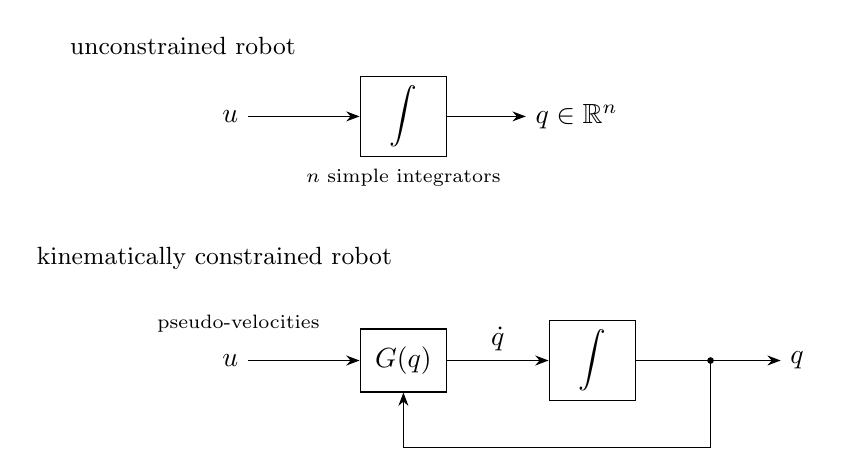
\begin{tikzpicture}[>=Stealth,box/.style={draw,minimum width=1.1cm,minimum height=0.8cm}]
% unconstrained
\node at (-0.6,0.9) {\small unconstrained robot};
\node (u1) at (0,0) {$u$};
\node[box] (I1) at (2.2,0) {$\displaystyle\int$};
\node (q1) at (4.4,0) {$q\in\R^n$};
\draw[->] (u1)--(I1);
\draw[->] (I1)--(q1);
\node[font=\scriptsize,below=1pt of I1] {$n$ simple integrators};
% constrained
\begin{scope}[yshift=-3.1cm]
\node at (-0.2,1.3) {\small kinematically constrained robot};
\node (u2) at (0,0) {$u$};
\node[box] (G) at (2.2,0) {$G(q)$};
\node[box] (I2) at (4.6,0) {$\displaystyle\int$};
\node (q2) at (7.2,0) {$q$};
\draw[->] (u2)--(G) node[midway,above,font=\scriptsize]{\strut};
\draw[->] (G)--(I2) node[midway,above]{$\dq$};
\draw[->] (I2)--(q2);
\fill (6.1,0) circle(1.2pt);
\draw[->] (6.1,0)--(6.1,-1.1)--(2.2,-1.1)--(G.south);
\node[font=\scriptsize,above=1pt of u2,xshift=3pt] {pseudo-velocities};
\end{scope}
\end{tikzpicture}
\caption{Block schemes of the kinematic model.}
\end{figure}

% =====================================================================
\section{Controllability of kinematic models}\emph{(page 4)}
% =====================================================================

\begin{definition}[Controllable KM]
A kinematic model is \emph{controllable} if for any initial configuration $q_i$ and any final configuration $q_f$ there exist a time $T$ and an input $u:[0,T]\to\R^m$ such that the solution of $\dq=G(q)u$ starting at $q_i$ reaches $q_f$ at time $T$.
\end{definition}

Controllability can be established in two ways: \emph{constructively}, by looking for a \emph{universal maneuver} that connects any pair of configurations, or by applying a \emph{test for controllability} (a rank condition, see Remark~\ref{rem:chow}).

\paragraph{Link with the constraints.} The notes relate controllability to the integrability of the kinematic constraints:
\begin{itemize}[nosep]
\item the KM is controllable $\iff$ the KCs are \emph{nonholonomic} (not integrable);
\item the KM is not controllable $\iff$ the KCs are \emph{holonomic}, i.e.\ integrable (partially or completely).
\end{itemize}

\begin{intuition}
If a constraint is integrable, it can be rewritten as a restriction on positions, $h(q)=\text{const}$ (for example $y=0$): the robot is trapped on a lower-dimensional surface and can never reach the other configurations, so the KM cannot be controllable. If the constraints are not integrable they leave the robot able to reach every configuration by sequencing admissible motions, as a car does when parallel parking: it cannot move sideways instantaneously, but it can reach any pose.
\end{intuition}

% =====================================================================
\section{The unicycle}\emph{(pages 4--6)}
% =====================================================================

\begin{definition}[Unicycle]
The unicycle is a vehicle with a single \emph{orientable} wheel. Its configuration is $q=(x,y,\theta)^{\!\top}$, where $(x,y)$ is the contact point and $\theta$ the orientation of the wheel's \emph{sagittal axis} with respect to the $x$-axis. The configuration space is $\mathcal{C}=\R^2\times \SO(2)$, locally $\simeq\R^3$ (hence $n=3$).
\end{definition}

\begin{figure}[h]
\centering
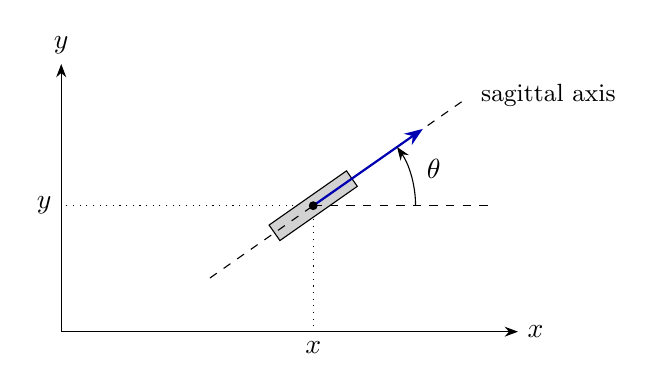
\begin{tikzpicture}[>=Stealth,scale=1]
\coordinate (P) at (3.2,1.6);
\draw[->] (0,0)--(5.8,0) node[right]{$x$};
\draw[->] (0,0)--(0,3.4) node[above]{$y$};
\draw[dotted] (P)--(3.2,0) node[below]{$x$};
\draw[dotted] (P)--(0,1.6) node[left]{$y$};
\begin{scope}[shift={(P)},rotate=35]
  \draw[fill=gray!35] (-0.6,-0.12) rectangle (0.6,0.12);
  \draw[dashed] (-1.6,0)--(2.4,0);
\end{scope}
\node[font=\small,anchor=west] at ($(P)+(35:2.45)$) {sagittal axis};
\draw[->,thick,blue!70!black] (P)--++(35:1.7) node[above]{};
\draw[dashed] (P)--++(2.3,0);
\draw[->] ($(P)+(1.3,0)$) arc (0:35:1.3);
\node at ($(P)+(17:1.6)$) {$\theta$};
\fill (P) circle(1.6pt);
\end{tikzpicture}
\caption{The unicycle seen from above: contact point $(x,y)$, sagittal axis at angle $\theta$.}
\end{figure}

\subsection{The pure rolling constraint}\emph{(page 5)}

The wheel rolls without slipping, so the contact point cannot move along the wheel axis (orthogonal to the sagittal axis):
\[
\sin\theta\,\dot x-\cos\theta\,\dot y=0 .
\]
Equivalently, $(\dot x,\dot y)$ must be \emph{aligned with the sagittal axis}, i.e.\ it has no component along the direction orthogonal to it. In Pfaffian form
\[
\underbrace{\begin{pmatrix}\sin\theta & -\cos\theta & 0\end{pmatrix}}_{A(q)}\begin{pmatrix}\dot x\\ \dot y\\ \dot\theta\end{pmatrix}=0,\qquad k=1,\ n=3,\ m=n-k=2 .
\]

\begin{intuition}
Worked numbers. At $\theta=0$: $A=(0,-1,0)$, so the constraint reads $\dot y=0$: the wheel may translate along $x$ and spin in place, never sideways. At $\theta=\pi/2$: $A=(1,0,0)$, so $\dot x=0$: now it may move along $y$ only. The forbidden direction rotates together with the wheel.
\end{intuition}

\begin{proposition}[Basis of the admissible velocities]\label{prop:basis}
A basis of $\N\big((\sin\theta\ \ {-\cos\theta}\ \ 0)\big)$, a 2-dimensional linear space, is
\[
g_1(q)=\begin{pmatrix}\cos\theta\\ \sin\theta\\ 0\end{pmatrix},\qquad g_2(q)=\begin{pmatrix}0\\0\\1\end{pmatrix}.
\]
\end{proposition}
\begin{proof}
$A g_1=\sin\theta\cos\theta-\cos\theta\sin\theta=0$ and $Ag_2=0$. The two vectors are linearly independent for every $\theta$, and $\dim\N(A)=3-1=2$.
\end{proof}

\paragraph{Kinematic model of the unicycle.}
\[
\dq=\begin{pmatrix}\cos\theta\\ \sin\theta\\ 0\end{pmatrix}u_1+\begin{pmatrix}0\\0\\1\end{pmatrix}u_2
\quad\Longleftrightarrow\quad
\begin{cases}\dot x=\cos\theta\,u_1\\ \dot y=\sin\theta\,u_1\\ \dot\theta=u_2 .\end{cases}
\]

\subsection{Interpretation of the inputs}\emph{(pages 5--6)}

From the model, $\dot x^2+\dot y^2=\cos^2\theta\,u_1^2+\sin^2\theta\,u_1^2=u_1^2$, hence
\[
u_1=\pm\sqrt{\dot x^2+\dot y^2}\quad(\text{equivalently }u_1=\cos\theta\,\dot x+\sin\theta\,\dot y),
\]
the magnitude of the velocity of the contact point, with sign $+$ for forward and $-$ for backward motion. We therefore rename
\[
u_1=v\ \text{(driving velocity)},\qquad u_2=\dot\theta=\omega\ \text{(steering velocity)} .
\]
The driving velocity is related to the angular velocity of the wheel about its own axis by $v=r\,\omega_{\rm roll}$ ($r$ = wheel radius, side view in Fig.~\ref{fig:wheel}); $\omega$ is the angular velocity of the wheel about the vertical axis.

\begin{definition}[Unicycle kinematic model]
\[
\dq=\begin{pmatrix}\cos\theta\\ \sin\theta\\ 0\end{pmatrix}v+\begin{pmatrix}0\\0\\1\end{pmatrix}\omega,
\qquad\text{i.e.}\quad
\begin{cases}\dot x=v\cos\theta\\ \dot y=v\sin\theta\\ \dot\theta=\omega .\end{cases}
\]
\end{definition}

\begin{figure}[h]
\centering
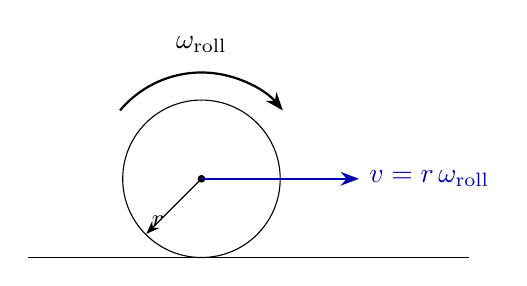
\begin{tikzpicture}[>=Stealth]
\draw (0,0) circle(1);
\fill (0,0) circle(1.4pt);
\draw[->] (0,0)--(-0.7,-0.7) node[midway,below left,font=\small]{$r$};
\draw[->,thick] (140:1.35) arc (140:40:1.35);
\node at (90:1.7) {$\omega_{\rm roll}$};
\draw (-2.2,-1)--(3.4,-1);
\draw[->,thick,blue!70!black] (0,0)--(2,0) node[right]{$v=r\,\omega_{\rm roll}$};
\end{tikzpicture}
\caption{Side view of the wheel: the driving velocity is $v=r\,\omega_{\rm roll}$.}\label{fig:wheel}
\end{figure}

\begin{intuition}
The basis $\{g_1,g_2\}$ was chosen so that the inputs are exactly what a driver feels: $v$ is ``how fast I roll along where I am pointing'' and $\omega$ is ``how fast I turn''. Any other basis (Proposition~\ref{prop:nonuniq}) would give an equivalent but less readable model. Constant inputs give circles: with $v=1\ \mathrm{m/s}$ and $\omega=0.5\ \mathrm{rad/s}$ the contact point moves on a circle of radius $v/\omega=2\ \mathrm m$ (see the figure in the Summary).
\end{intuition}

% =====================================================================
\section{Controllability of the unicycle}\emph{(page 7)}
% =====================================================================

\begin{proposition}\label{prop:unicycle-ctrl}
The unicycle KM is controllable: it can be steered from any $q_i=(x_i,y_i,\theta_i)$ to any $q_f=(x_f,y_f,\theta_f)$.
\end{proposition}

The notes answer ``yes'' by applying a universal maneuver, the same idea used earlier for the disk, in three steps.

\begin{algorithm}[Universal maneuver for the unicycle]\label{alg:maneuver}
Let $\varphi=\operatorname{atan2}(y_f-y_i,\ x_f-x_i)$ and $d=\sqrt{(x_f-x_i)^2+(y_f-y_i)^2}$.
\begin{enumerate}[nosep]
\item $v=0$, $\omega=$ constant, until $\theta=\varphi$ (rotate in place to point at the goal).
\item $v=$ constant, $\omega=0$, until $(x,y)=(x_f,y_f)$ (drive straight, distance $d$).
\item $v=0$, $\omega=$ constant, until $\theta=\theta_f$ (rotate in place to the final orientation).
\end{enumerate}
\end{algorithm}

\begin{proof}[Proof of Proposition~\ref{prop:unicycle-ctrl}]
During phases 1 and 3, $v=0$ gives $\dot x=\dot y=0$ and $\dot\theta=\omega$, so the position is frozen and $\theta$ changes at will; phase 1 takes $\theta$ from $\theta_i$ to $\varphi$ in time $T_1=(\varphi-\theta_i)/\omega$. During phase 2, $\omega=0$ keeps $\theta=\varphi$ constant, so $(\dot x,\dot y)=v(\cos\varphi,\sin\varphi)$ is a straight line, reaching $(x_f,y_f)$ after $T_2=d/v$. Phase 3 takes $\theta$ from $\varphi$ to $\theta_f$. (If $d=0$ phase 2 is skipped.)
\end{proof}

\begin{figure}[h]
\centering
\begin{tikzpicture}[>=Stealth,scale=1]
\coordinate (I) at (0,0);\coordinate (F) at (5.2,3);
\fill (I) circle(1.6pt) node[below left]{$q_i$};
\fill (F) circle(1.6pt) node[above right]{$q_f$};
\draw[->,thick] (I)--++(-20:1.0) node[right]{$\theta_i$};
\draw[dashed] (I)--(F);
\draw[->,very thick,blue!70!black] ($(I)+(-20:0.65)$) arc(-20:30:0.65);
\node[blue!70!black] at ($(I)+(5:0.95)$) {\small\textcircled{\scriptsize1}};
\draw[->,very thick,red!70!black] ($(I)!0.25!(F)$)--($(I)!0.75!(F)$);
\node[red!70!black,above left] at ($(I)!0.5!(F)$) {\small\textcircled{\scriptsize2}};
\draw[->,very thick,blue!70!black] ($(F)+(30:0.65)$) arc(30:100:0.65);
\node[blue!70!black] at ($(F)+(65:1.0)$) {\small\textcircled{\scriptsize3}};
\draw[->,thick] (F)--++(100:1.0) node[above]{$\theta_f$};
\end{tikzpicture}
\caption{Universal maneuver: rotate in place, drive straight, rotate in place.}
\end{figure}

\begin{intuition}
It is a ``point, drive, align'' strategy. Worked numbers: from $q_i=(0,0,0)$ to $q_f=(3,4,\pi/2)$ we have $\varphi=\arctan(4/3)\approx0.927$ rad ($53.1^\circ$) and $d=5$. With $|\omega|=1$ rad/s and $v=1$ m/s: rotate for $0.927$ s, drive for $5$ s, rotate for $\pi/2-0.927\approx0.644$ s ($36.9^\circ$). The two rotations ``cost'' nothing in position, which is possible only because the model lets us set $v=0$ and turn freely.
\end{intuition}

\begin{intuition}[Consistency with Section 3]
Despite the constraint $\dot y=0$ at $\theta=0$ (no sideways motion), the unicycle can reach any pose, because the pure rolling constraint is \emph{not integrable}: this is exactly the controllable/nonholonomic case.
\end{intuition}

\begin{lemma}[Rank test, supplementary]\label{rem:chow}
Let $[g_1,g_2]=\frac{\partial g_2}{\partial q}g_1-\frac{\partial g_1}{\partial q}g_2$ be the Lie bracket. For the unicycle $[g_1,g_2]=(\sin\theta,\,-\cos\theta,\,0)^{\!\top}$, and $\rank\{g_1,g_2,[g_1,g_2]\}=3=n$ for every $q$, so the controllability rank condition (Chow) holds.
\end{lemma}
\begin{proof}
$\partial g_2/\partial q=0$ and $\partial g_1/\partial q\,g_2=(-\sin\theta,\cos\theta,0)^{\!\top}$, hence $[g_1,g_2]=(\sin\theta,-\cos\theta,0)^{\!\top}$, which is orthogonal to $g_1$ and independent of $g_2$.
\end{proof}
\noindent\emph{(This is the ``test for controllability'' mentioned on page 4; the explicit computation is not in the handwritten notes.)}

\begin{intuition}
$[g_1,g_2]$ points \emph{sideways}, exactly the forbidden direction: the wiggle ``drive, turn, back up, turn back'' produces a net sideways displacement, the same effect as parallel parking.
\end{intuition}

% =====================================================================
\section{Mechanically equivalent vehicles}\emph{(pages 7--8)}
% =====================================================================

Several real vehicles have the unicycle KM as soon as the right inputs are chosen.

\subsection{Differential drive}\emph{(page 7)}

Two parallel wheels (left and right) with a common axis; the reference point is the \emph{midpoint between the two contact points}. Its KM is the unicycle one,
\[
\begin{cases}\dot x=\cos\theta\,v\\ \dot y=\sin\theta\,v\\ \dot\theta=\omega\end{cases}
\qquad
v=r\,\frac{\omega_R+\omega_L}{2},\qquad \omega=r\,\frac{\omega_R-\omega_L}{d},
\]
where $\omega_R,\omega_L$ are the roll velocities of the right and left wheel, $r$ the wheel radius and $d$ the distance between the wheels (the denominator is cut off in the handwritten page).

\begin{proposition}
For a differential drive, the physical inputs $(\omega_R,\omega_L)$ are related to the unicycle inputs $(v,\omega)$ by an invertible linear map.
\end{proposition}
\begin{proof}
The contact points move with speeds $v_R=r\omega_R$ and $v_L=r\omega_L$. The midpoint has velocity $v=(v_R+v_L)/2$ and the body rotates with $\omega=(v_R-v_L)/d$. The matrix $\frac r2\begin{pmatrix}1&1\\ 2/d&-2/d\end{pmatrix}$ has determinant $-2r^2/d\neq0$.
\end{proof}

\begin{figure}[h]
\centering
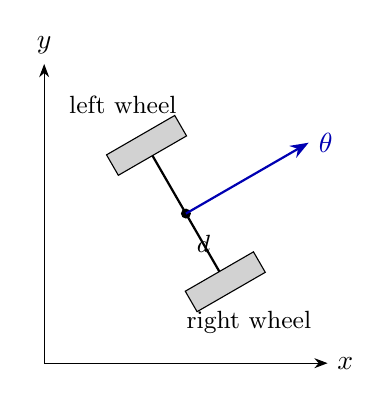
\begin{tikzpicture}[>=Stealth]
\coordinate (M) at (0,0);
\draw[->] (-1.8,-1.9)--(1.8,-1.9) node[right]{$x$};
\draw[->] (-1.8,-1.9)--(-1.8,1.9) node[above]{$y$};
\begin{scope}[rotate=30]
  \draw[thick] (0,-1)--(0,1);
  \draw[fill=gray!35] (-0.5,0.85) rectangle (0.5,1.15);
  \draw[fill=gray!35] (-0.5,-1.15) rectangle (0.5,-0.85);
\end{scope}
\fill (M) circle(1.8pt);
\draw[->,thick,blue!70!black] (M)--++(30:1.8) node[right]{$\theta$};
\node[font=\small] at ($(M)+(120:1.6)$) {left wheel};
\node[font=\small] at ($(M)+(-60:1.6)$) {right wheel};
\node[font=\small] at ($(M)+(-60:0.45)$) {$d$};
\end{tikzpicture}
\caption{Differential drive seen from above; the reference point is the midpoint of the axle.}
\end{figure}

\begin{intuition}
Worked numbers: $r=0.1$ m, $d=0.4$ m, $\omega_R=10$ rad/s, $\omega_L=6$ rad/s. Then $v=0.1\cdot16/2=0.8$ m/s and $\omega=0.1\cdot4/0.4=1$ rad/s, a turn of radius $v/\omega=0.8$ m. Equal wheel speeds give $\omega=0$ (straight line); opposite speeds give $v=0$ (rotation in place, the first and third phase of the universal maneuver).
\end{intuition}

\subsection{Synchro-drive}\emph{(page 8)}

A synchro-drive has three (or more) wheels that are steered and driven in a synchronized way, so that all wheels always point in the same direction $\theta$. The notes state that the KM \emph{is} the unicycle one and that \emph{no input transformation is needed}:
\[
\begin{cases}\dot x=\cos\theta\,v\\ \dot y=\sin\theta\,v\\ \dot\theta=\omega ,\end{cases}
\]
with $v$ the common driving velocity and $\omega$ the common steering velocity.

\begin{figure}[h]
\centering
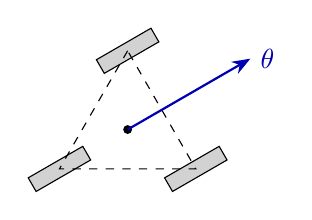
\begin{tikzpicture}[>=Stealth]
\coordinate (M) at (0,0);
\foreach \a in {90,210,330}{
  \begin{scope}[shift={(\a:1)},rotate=30]
    \draw[fill=gray!35] (-0.4,-0.1) rectangle (0.4,0.1);
  \end{scope}
}
\draw[dashed] (90:1)--(210:1)--(330:1)--cycle;
\fill (M) circle(1.6pt);
\draw[->,thick,blue!70!black] (M)--++(30:1.8) node[right]{$\theta$};
\end{tikzpicture}
\caption{Synchro-drive: three wheels steered together, all with orientation $\theta$.}
\end{figure}

\begin{intuition}
Because every wheel is always aligned with the others, the vehicle behaves as one big unicycle: the \emph{body orientation} that the model calls $\theta$ is the common steering angle. Unlike the differential drive, the physical inputs (driving and steering velocity of the synchronized wheels) already coincide with $(v,\omega)$, so the model works as is.
\end{intuition}

% =====================================================================
\section{Summary}
% =====================================================================

\begin{table}[h]
\centering\small
\renewcommand{\arraystretch}{1.25}
\begin{tabular}{@{}p{2.9cm}p{1.2cm}p{1.2cm}p{1.2cm}p{3.3cm}p{3.2cm}@{}}
\toprule
\textbf{System} & $\boldsymbol n$ & $\boldsymbol k$ & $\boldsymbol m$ & \textbf{Inputs $u$} & \textbf{Model}\\
\midrule
Unconstrained robot & $n$ & $0$ & $n$ & $u\in\R^n$ (fully actuated) & $\dq=u$ (canonical basis)\\
Unicycle & $3$ & $1$ & $2$ & $v$ (driving), $\omega$ (steering) & $\dq=g_1v+g_2\omega$\\
Differential drive & $3$ & $1$ & $2$ & $\omega_R,\omega_L\Rightarrow v=r\frac{\omega_R+\omega_L}2,\ \omega=r\frac{\omega_R-\omega_L}d$ & unicycle KM\\
Synchro-drive & $3$ & $1$ & $2$ & $v,\omega$ directly (no transformation) & unicycle KM\\
\bottomrule
\end{tabular}
\caption{Kinematic models covered. All are driftless and nonlinear in $q$; the three wheeled vehicles are controllable.}
\end{table}

\begin{figure}[h]
\centering
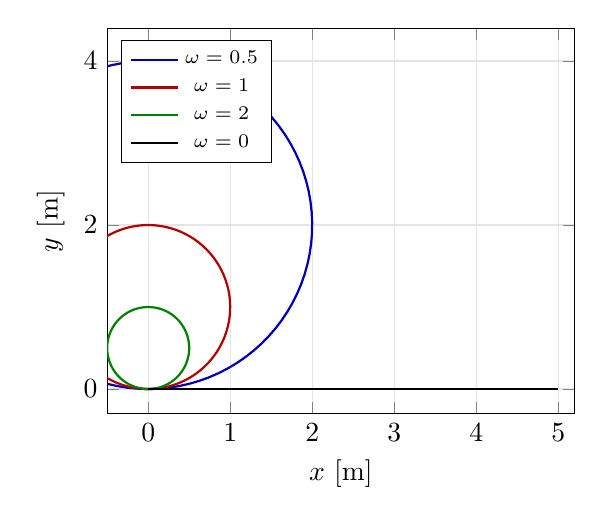
\begin{tikzpicture}
\begin{axis}[width=0.62\linewidth,axis equal image,xlabel={$x$ [m]},ylabel={$y$ [m]},
  xmin=-0.5,xmax=5.2,ymin=-0.3,ymax=4.4,legend pos=north west,legend style={font=\scriptsize},
  grid=both,grid style={gray!20}]
\addplot[blue!70!black,thick,domain=0:2*pi,samples=100] ({2*sin(deg(x))},{2*(1-cos(deg(x)))});
\addplot[red!70!black,thick,domain=0:2*pi,samples=100] ({1*sin(deg(x))},{1*(1-cos(deg(x)))});
\addplot[green!50!black,thick,domain=0:2*pi,samples=100] ({0.5*sin(deg(x))},{0.5*(1-cos(deg(x)))});
\addplot[black,thick] coordinates {(0,0)(5,0)};
\legend{$\omega=0.5$,$\omega=1$,$\omega=2$,$\omega=0$}
\end{axis}
\end{tikzpicture}
\caption{Unicycle with $v=1$ m/s, $q_i=(0,0,0)$ and constant $\omega$: circles of radius $v/\omega$ (straight line for $\omega=0$).}
\end{figure}

\subsection*{Key take-aways}
\begin{itemize}
\item Wheels impose Pfaffian constraints $A(q)\dq=0$; admissible velocities form $\N(A(q))$, of dimension $m=n-k$.
\item The kinematic model $\dq=G(q)u$ is a nonlinear, driftless system; $G$ is not unique, and bases are chosen for interpretability.
\item The unicycle ($n=3,k=1,m=2$) has $\dot x=v\cos\theta,\ \dot y=v\sin\theta,\ \dot\theta=\omega$; $v=r\omega_{\rm roll}$ is the driving velocity and $\omega$ the steering velocity.
\item Controllability of a KM is tied to nonholonomy of the constraints; the unicycle is controllable via the \emph{rotate--drive--rotate} maneuver.
\item Differential drive and synchro-drive share the unicycle KM (the former after the linear input change $v=r\frac{\omega_R+\omega_L}2$, $\omega=r\frac{\omega_R-\omega_L}d$).
\end{itemize}

\end{document}